\documentclass[12pt,letterpaper]{article}
\usepackage[left=1.22in,right=1.22in,top=0.84in,bottom=0.82in,headheight=15pt]{geometry}
\usepackage[T1]{fontenc}
\usepackage{lmodern,microtype,graphicx,booktabs,array,amsmath,amssymb}
\usepackage[dvipsnames]{xcolor}
\usepackage{tikz}
\usetikzlibrary{arrows.meta,positioning,fit,calc}
\usepackage[round,authoryear]{natbib}
\usepackage[colorlinks=true,urlcolor=NavyBlue,citecolor=NavyBlue,linkcolor=NavyBlue]{hyperref}
\usepackage{fancyhdr}
\usepackage{enumitem}
\setlist{nosep,leftmargin=1.45em}
\setlength{\parindent}{0pt}
\setlength{\parskip}{0.56em}
\setlength{\emergencystretch}{2em}
\renewcommand{\baselinestretch}{1.15}
\pagestyle{fancy}
\fancyhf{}
\fancyhead[L]{\small\textsc{Authorized Agent Workflows}}
\fancyhead[R]{\small newdarwindev}
\fancyfoot[C]{\thepage}
\renewcommand{\headrulewidth}{0.3pt}
\newcommand{\keypoint}[1]{\vspace{0.35em}\noindent\colorbox{NavyBlue!7}{\parbox{0.94\linewidth}{\small\textbf{Design claim.} #1}}\vspace{0.35em}}
\newcommand{\nextpage}{\clearpage}
\title{\Huge\bfseries Authorized Agent Workflows\\[0.35em]\Large A Research Agenda for Turning General Models into Valuable, Permitted Work}
\author{newdarwindev}
\date{October 2026}
\begin{document}
\maketitle
\thispagestyle{empty}
\vspace{0.3in}
\begin{abstract}
This position paper argues that a particularly large commercial research opportunity for teams outside frontier model laboratories is to make widely available models complete valuable, owner-authorized tasks across accounts, browsers, APIs, and human checkpoints. The claim is a strategic hypothesis, not a measured ranking of research opportunities. Many apparent model failures are failures of integration, authority, durable execution, or permission rather than reasoning alone. We propose a task model that separates those causes, an architecture that places credentials and policy outside model context, and an evaluation protocol centered on successful authorized outcomes, human effort, and total cost. Account enrollment, credential custody, and social publishing are treated as permissioned workflows with explicit human handoff and platform compliance. The paper offers falsifiable predictions, competing explanations, and a research agenda; it reports no deployed system or measured business return.
\end{abstract}
\vfill
\begin{center}
\begin{minipage}{0.86\linewidth}
\small\textbf{Audience:} applied AI researchers, product engineers, and technical founders.\\
\textbf{Scope:} systems design and evaluation for legitimate owner-authorized automation.\\
\textbf{Status:} conceptual proposal; all architecture components are illustrative.
\end{minipage}
\end{center}
\vspace{0.35in}
\nextpage

\section{The commercial thesis}
General models can write a plan, call tools, and interpret screens. Yet a consumer product often stops before an economically meaningful outcome: a verified account, an approved publication, an updated record, or a safely reconciled transaction. The gap is attractive to researchers who cannot train a frontier model because the missing work may be in the surrounding system: identity, permissions, state, observability, and recovery. A model can be strong enough to choose a next step while the product remains unable to execute that step with legitimate authority.

Our thesis is deliberately strong: for some applied teams, the greatest near-term commercial research opportunity may be the engineering of these authorized workflows around consumer-level frontier models. ``Greatest'' is a comparative hypothesis requiring evidence against model improvement, deterministic software, vertical SaaS, and other agent opportunities. The paper does not claim such evidence already exists. It claims the hypothesis deserves a serious test because completion across real systems is a distinct research problem from next-token accuracy or isolated tool-use success.

This thesis has a boundary. A refusal may express a safety policy or a platform restriction that should remain in force. The useful opportunity concerns tasks an owner is entitled to perform and a product is permitted to support, where a workflow can provide missing integration or supervised handoff. The work is not to extract a yes from a model that correctly says no. It is to find the lawful, authorized execution path and to represent ``no available path'' as a legitimate outcome.

WebArena, WorkArena, OSWorld, and BrowserGym document how difficult end-to-end interaction can be in benchmark environments \citep{webarena,workarena,osworld,browsergym}. Their task distributions do not measure a market. They motivate methods for evaluating multi-step outcomes, not a numerical claim about present-day deployment performance. A viable research program must observe whether completion and economic value improve after adding authority-aware infrastructure, holding the model and task set fixed.

\keypoint{The object of study is the full authorized task, including handoff and recovery, rather than a model's ability to produce plausible action text.}
\nextpage

\section{Five causes of noncompletion}
The phrase ``the model refuses'' conflates different mechanisms. We distinguish five causes because each suggests a different intervention and a different ethical answer. First, \emph{capability failure}: the model misunderstands a page, loses context, or chooses the wrong action. Better models, perception, or planning may help. Second, \emph{integration failure}: the model can describe the right action but has no reliable tool, browser state, API scope, or durable executor. A connector or orchestrator may help.

Third, \emph{authorization failure}: the user has not granted the right account, scope, or specific approval for an effect. The right response is a request to the owner or an authorized administrator, not inferred consent. Fourth, \emph{product or safety refusal}: the provider or application disallows the request even if a tool exists. Researchers should record this as a boundary, not hide it as a tool error. Fifth, \emph{third-party platform restriction}: a service may prohibit particular automation or require a reviewed API, rate limit, consent flow, or human operation. OAuth possession alone does not settle that question; platform rules are separate from technical access \citep{slackoauth,xrules,linkedinrules}.

The classes can overlap. A login page may combine an unavailable browser session, a missing delegated scope, and an identity check reserved for a person. An evaluation should assign a primary cause and secondary factors at each blocked transition. This diagnostic record prevents a system from celebrating an apparent completion that simply shifted responsibility or violated a service rule. It also tells a builder where investment belongs: prompts for reasoning errors, APIs for integration, approval flows for authority, or an explicit stop for a disallowed action.

The operational definition of ``valuable task'' should be a user-recognizable terminal state, independently checked where possible. A draft is not a published post; a filled form is not an accepted registration; a tool call is not a confirmed update. Researchers should specify the intended terminal state before the run and distinguish it from partial work, pending human review, and terminal noncompletion. This is essential for comparing systems that delegate difficult steps to humans at different points.

\keypoint{Classify the blocked transition before trying to solve it; some blocks are constraints to preserve.}
\nextpage

\section{A task, authority, and state model}
Let a task be $T=(g,E,A,P,B)$: goal $g$, external environment $E$, authority record $A$, policy set $P$, and resource budget $B$. The environment has partially observable state $s_t$; the system receives observations $o_t$ and proposes actions $a_t$. The authority record binds a principal, resource, scope, purpose, expiry, and approval state. A proposed action is executable only if it is both technically available and permitted by $A$ and $P$ at time $t$. A human approval is a new event, not a prediction that approval would probably be given.

We write a transition as $s_{t+1}\sim F(s_t,a_t)$, but external effects can be uncertain. A timeout after ``submit'' does not imply the action failed. Thus the state must include a local event journal, evidence of remote effects, and an explicit \emph{unknown} outcome. The workflow may retry a pure read, but it must reconcile an uncertain write before another attempt. This is especially important when an effect is expensive, public, or difficult to reverse.

Success has three parts: the requested goal is reached; the path obeys permissions; and the evidence is adequate to support the claim. Formally, $Y=1$ only if $G(s_f)=1$, $\operatorname{Allowed}(a_{1:f},A,P)=1$, and $\operatorname{Verified}(s_f)=1$. An agent that produces the right looking output using an unapproved credential fails the task under this definition. The same applies when a workflow asserts completion from a click without checking the remote state.

An authority record is narrower than a user saying ``handle my accounts.'' It should identify the account and action classes, separate read from write, express irreversible effects, and expire. It can be renewed with a fresh approval. The model receives a capability handle or tool description, never a general right to improvise access. This formalization is intentionally minimal; policy law and vendor terms remain external inputs to a real deployment. The research question is whether such explicit authority reduces invalid actions while preserving useful completion.

\keypoint{A correct goal reached through an unauthorized path is a failure, and an unverified remote state is an unknown.}
\nextpage

\section{An illustrative integration architecture}
Figure~\ref{fig:architecture} sketches a proposed system, not a deployed prototype. A request enters an authority registry and policy gate before a model planner receives tools. The planner emits bounded intents to a durable workflow, which invokes API or browser adapters. A credential broker leases or retrieves the minimum material needed by an adapter; the planner sees neither the secret nor the browser's raw storage state. A human station handles identity checks, consequential approvals, and ambiguous outcomes. The evidence journal records observed state and correlates actions with approvals.

\begin{figure}[h]
\centering
\resizebox{0.96\linewidth}{!}{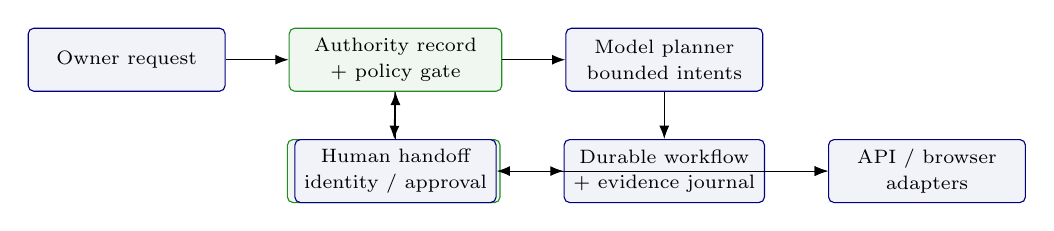
\begin{tikzpicture}[>=Latex, node distance=6mm and 8mm, every node/.style={font=\scriptsize},
  box/.style={draw=NavyBlue,rounded corners=2pt,fill=NavyBlue!5,align=center,minimum height=8mm,minimum width=25mm},
  gate/.style={draw=ForestGreen,rounded corners=2pt,fill=ForestGreen!7,align=center,minimum height=8mm,minimum width=27mm}]
\node[box] (owner) {Owner request};
\node[gate,right=of owner] (auth) {Authority record\\+ policy gate};
\node[box,right=of auth] (planner) {Model planner\\bounded intents};
\node[box,below=of planner] (flow) {Durable workflow\\+ evidence journal};
\node[gate,left=of flow] (broker) {Credential broker\\scoped retrieval};
\node[box,right=of flow] (adapter) {API / browser\\adapters};
\node[box,below=of auth] (human) {Human handoff\\identity / approval};
\draw[->] (owner) -- (auth);
\draw[->] (auth) -- (planner);
\draw[->] (planner) -- (flow);
\draw[->] (flow) -- (adapter);
\draw[->] (broker) -- (adapter);
\draw[->] (auth) -- (broker);
\draw[<->] (flow) -- (human);
\draw[->] (human) -- (auth);
\end{tikzpicture}
}
\caption{Proposed separation of planning, authority, execution, human handoff, and evidence. Arrows denote controlled calls or state transitions, not implicit trust.}
\label{fig:architecture}
\end{figure}

OpenBao could serve as a secret store, Temporal as a durable workflow engine, and a controlled browser as one adapter. PinchTab, KasmVNC, Authelia, Pomerium, or Caddy are possible public components for browser control, human access, identity, or ingress; naming them does not assert security or performance of the combined design. An implementation should choose components only after threat modeling and operational testing. In particular, a browser session and a model tool channel must be scoped separately. The network boundary is not the authority boundary.

The architecture makes an important allocation of work. Deterministic code validates scopes, enforces rate limits, persists events, and applies idempotency keys where the external API offers them. A model interprets unstructured instructions and changing interface content. Humans perform acts that demand personal identity or judgment. These roles can change by task, but the interfaces should make the change explicit. The integration itself is a research artifact because it exposes failure modes that isolated model tests do not.
\nextpage

\section{Credential custody outside model context}
Credential marshalling means obtaining an authorized credential, placing it in appropriate custody, supplying it only to an allowed tool for a bounded purpose, and rotating or revoking it when possible. This is more than copying a password into a prompt. The model should receive a reference to an action capability, while a broker decides whether the current task and principal may use the underlying secret. Logs and traces must exclude raw secret values, browser cookies, and authorization headers.

An owner might connect an official OAuth application, grant a short-lived token with narrow scopes, or place an existing service secret in a vault. Those paths have different risk. OAuth grants can often be scoped and revoked at the provider; an ordinary website password stored in a KV secret engine is still a long-lived password. OpenBao's lease mechanism applies to generated or leased credentials, not automatically to arbitrary KV values \citep{openbaolease,openbaodb}. The design must not claim that vault storage itself makes a website password dynamically revocable.

A broker should bind each retrieval to a principal, task identifier, approved tool, destination, time window, and purpose. It should decline a destination mismatch and record the decision without logging the secret. When a third-party API supports a narrower token, prefer it over a full account session. A browser adapter may need session state; Playwright documentation cautions that stored authentication state can contain cookies or headers able to impersonate the user \citep{playwrightauth}. Such state must be kept out of the public repository and out of model-readable artifacts.

This externalization can itself fail. Secret custody creates an attractive target and operational duties: access review, incident response, revocation, and audit. A builder should compare its residual risk with user-operated handoff or an official integration that avoids storing secrets altogether. The research payoff is conditional: lower human friction is valuable only if the custody system stays permissioned and manageable.

\keypoint{A vault reduces exposure to the model; it does not create authority or transform every secret into a revocable lease.}
\nextpage

\section{Account enrollment and human verification}
Account registration is an unusually clear test of the distinction between preparation and authority. An assistant may gather public requirements, draft profile fields supplied by an owner, navigate to the official enrollment flow, and preserve progress. A person should supply identity assertions, verify email or phone access, complete any site-required challenge, and accept binding terms when required. The workflow can resume after those events are reported as human actions. It should not claim registration merely because a form was filled.

The task state should include \emph{prepared}, \emph{awaiting owner}, \emph{submitted}, \emph{pending review}, \emph{verified}, and \emph{failed}. These states matter commercially: they let a product say what remains to be done and avoid starting the same enrollment twice. They also let an evaluator count human minutes and waiting time separately. A system that moves a ten-minute form into a one-minute agent step but leaves a long verification queue has not necessarily improved the full outcome.

Human handoff should be bounded. The agent provides the person the exact site, purpose, requested fields, and effect of confirmation; it never requests a one-time code in a chat transcript or a shared log. After the person finishes, the adapter re-reads the site or API to verify the account state. If a service supplies no reliable machine-readable status, a conservative terminal state is \emph{owner-confirmed, unverified by system}. That is useful progress but should not be scored as independently verified completion.

An account is not a commodity to create at scale without context. Eligibility, platform terms, rate limits, organization policy, and the service's own registration rules set the boundary. Many tasks will correctly end in a manual process or a refusal. Research should measure whether structured preparation and resumable state reduce owner effort for permitted enrollments, not whether the system can defeat friction intentionally imposed by the platform.

\keypoint{Treat personal verification and binding acceptance as explicit human events in the workflow state machine.}
\nextpage

\section{Social and publishing workflows}
Social publishing offers visible terminal states but demanding permission semantics. A legitimate workflow begins with a named owner, account, intended audience, content, timing, and platform-approved route. It may draft copy, route it for approval, use an official API with an authorized scope where available, and verify the published object. It should preserve the exact approved content or seek renewed approval for material changes. Posting, editing, deleting, following, messaging, and analytics reads are different action classes and should receive separate permissions.

Official APIs are not blanket permission. Slack's OAuth documentation describes scoped access, while platform-specific automation rules can add conditions beyond token possession \citep{slackoauth,xrules}. LinkedIn's help material describes restrictions on automated activity \citep{linkedinrules}. A product should encode the relevant platform rule as a deployment condition and re-evaluate it when rules change. If a permitted API is unavailable for a requested effect, human operation is a legitimate workflow branch. The system should not silently switch to brittle browser automation merely because it can click the same controls.

For publication, evidence should include a platform-provided object identifier or a durable public URL where appropriate, plus a post-action read. If the API call times out, the workflow first searches for the object or asks the owner to reconcile; it does not resubmit immediately. For a scheduled post, distinguish acceptance of a schedule from actual publication. For a draft, distinguish content approval from account authority. These distinctions prevent the demo-friendly but costly error of counting an intermediate artifact as the goal.

There is a business case for a narrow, compliant product: many teams need repeatable approvals, attribution, and audit trails around content that a general assistant can draft but cannot legitimately publish for them. Whether that case outruns existing software must be tested against a deterministic scheduler and a human-only baseline. The model is valuable when interpreting instructions or adapting drafts, not merely because a language model is in the loop.

\keypoint{Approval of content, authority over an account, and permission under platform rules are separate gates.}
\nextpage

\section{Browser state, observation, and handoff}
Browser automation is useful for tasks without a sufficient API, but it inherits fragile interface state. A page can change between observation and action; a button may appear twice; a login can expire; a modal can hide the target. The agent's observation should carry the page URL, origin, task context, and time, while the adapter executes against a fresh state. The system should prefer stable selectors and semantic labels, but it still needs to verify the resulting state after each consequential action.

Stored browser authentication is a credential. Playwright explicitly warns that authentication state may contain sensitive cookies and headers \citep{playwrightauth}. A useful architecture stores this state encrypted, scopes it to one principal and site, and prevents it from entering prompts, screenshots shipped to public logs, or source control. A browser controlled by both an owner and an agent needs explicit control transfer: pause the agent, show the current task and URL, let the owner act, then resume only after an event says control returned.

The handoff event should describe what the agent knows, what the person must decide, and what observation will indicate completion. It should not include instructions to type a code into an agent chat. For ambiguous remote effects, the system can invite the owner to inspect a page; its journal records the owner's report separately from machine verification. This separation makes postmortems possible when the remote site later disagrees with the owner's impression.

Prompt injection is another browser-state hazard: page text is untrusted content, not a new instruction from the owner. The Model Context Protocol security guidance describes confused-deputy and token-passthrough risks at tool boundaries \citep{mcpsecurity}. A browser adapter must not let a page request broader credentials, a new destination, or a changed workflow goal. The policy gate uses the pre-existing authority record, not instructions found in the page, to authorize every effect.

\keypoint{Treat browser content as observations and browser session state as a credential.}
\nextpage

\section{Durable execution and uncertain side effects}
Long tasks cross timeouts, worker restarts, owner absences, and external review queues. A durable workflow records the current task state and waits for events instead of asking a model to remember everything in a long transcript. A workflow can resume at a named step, reconstruct prior approvals, and make retries visible. Temporal's activity model is an example: an activity attempt may run again if completion was not recorded, even when an external effect occurred \citep{temporalactivity}. This is why ``durable'' does not mean exactly-once effects on a website.

Classify each step by side-effect risk. A pure read can usually be retried. A reversible write may use an idempotency key if the service supports it. A public or irreversible write needs precondition checks, effect evidence, and reconciliation. Suppose a publish call times out after the platform accepted it. Blind retry can create a duplicate. The workflow should query for an object matching a correlation key, examine platform response history, or pause for owner review. When neither path can establish state, retain \emph{unknown}; do not convert uncertainty into failure or success for a cleaner dashboard.

The event journal should contain intent, policy decision, tool call identifier, remote response metadata, verification observation, and any human event. It should retain only the data needed for audit and troubleshooting. In particular, avoid embedding raw credentials or unnecessary personal content. The goal is accountable progress, not total surveillance of every browser pixel. Retention and access rules are part of the system design.

Durability also changes evaluation. A benchmark that ends at a fixed short horizon misses delayed verification and recovery. A task should be scored after an explicit deadline, with states for completed, pending human action, pending platform action, failed, and unknown. This exposes whether orchestration reduces net work or merely extends the time until failure is recorded.

\keypoint{Every side-effecting step needs a retry policy tied to what the remote system can actually verify.}
\nextpage

\section{Policy as an executable boundary}
The policy gate should answer a narrow question: may this principal perform this action on this resource, for this purpose, now, through this route? It should read a versioned authority record and a versioned rule set. It should not ask the model to infer permissions from tone, urgency, or a webpage. The record can express allowed action classes, maximum scope, budget, rate, expiry, and whether another human must approve the specific effect.

A useful decision object has three outcomes: \emph{allow}, \emph{require approval}, or \emph{deny}. It contains the rule version and a short reason. ``Require approval'' is a suspended workflow state, not an automatic yes after a timeout. A denial is reportable without revealing private policy internals. When site terms or an organization's access policy are uncertain, the system should stop the effect and seek a responsible review rather than treating silence as permission.

Policies need to sit before secret retrieval and before effectful adapters. Otherwise a model could acquire a credential and then fail a later check, leaving a wider exposure than necessary. A low-level adapter should enforce destination and scope independently of the planner's proposed arguments. This is defense in depth, not an assertion that any single prompt or classifier is perfect. The MCP security guidance identifies token audience and confused-deputy issues that make this separation material \citep{mcpsecurity}.

The policy gate must also be testable. Researchers can construct cases where the same instruction changes outcome after a scope expires, an owner revokes access, the destination origin changes, or a platform rule forbids the route. Desired behavior is consistent denial or handoff, with no hidden side effects. A business product that cannot explain why an action was allowed cannot reliably satisfy an enterprise buyer's audit requirements. Yet explainability alone is insufficient: the system must prove the adapter received only the permitted capability.

\keypoint{Authority is checked at the effect boundary, with a specific decision recorded for each consequential step.}
\nextpage

\section{Threat model and trust boundaries}
The main assets are owner credentials, browser sessions, unpublished content, permission records, and evidence of remote effects. The adversarial surfaces include a malicious webpage, a compromised integration, a prompt injection in retrieved content, an unauthorized user, and an accidental operator mistake. The system must assume that a model may misunderstand text or overgeneralize an instruction even without an active attacker. These are separate threats requiring different controls.

The first boundary is from owner instruction to authority record. A user request can authorize a task, but ambiguous account names and broad verbs need resolution before sensitive effects. The second is from untrusted external content to model context; a page can describe data but cannot grant a new permission. The third is from model intent to tool execution; adapters validate destination, principal, and scope again. The fourth is from secret store to adapter; a secret is exposed only for the duration and destination of a permitted call. The fifth is from tool response to claimed outcome; a response is verified against the expected remote state.

Defense choices include scoped official APIs, least-privilege service accounts, human approval of consequential public effects, audit logs without secret values, session isolation, and revocation procedures. Browser use should be isolated from unrelated accounts. The system should test how it behaves when a site embeds an instruction to export tokens or when a tool returns a forged success message. Such tests are not demonstrations of bypass; they are checks that authority remains anchored outside untrusted content.

Residual risk remains substantial. A vault can be compromised; platform behavior can change; a human may approve the wrong content; an API can report success before publication is visible. The architecture therefore cannot promise risk elimination. It can make permissions explicit, reduce credential exposure to the model, create evidence for reconciliation, and make failures recoverable. These benefits must be measured against the added attack surface and operating cost of the infrastructure.

\keypoint{The model, the browser page, and the adapter have different trust levels; a single conversation does not collapse them.}
\nextpage

\section{Evaluation tasks and baselines}
The empirical test should use a task suite built from owner-authorized workflows in controlled accounts or service sandboxes. Tasks should cover credential connection, a permitted account enrollment with a human verification step, an approved content publication through an allowed API, a browser-only update that the service permits, and recovery after an uncertain side effect. Each task specification includes starting state, authority record, policy, goal predicate, deadline, and permitted human actions. No real owner secrets belong in a public benchmark.

Compare at least four systems under the same tasks: a human-only process, deterministic scripts with ordinary UI or API integrations, a model with tools but no durable authority-aware workflow, and the proposed workflow with the same model. A fifth condition can use a stronger model while holding the harness fixed. This factorial comparison isolates whether value comes from model capability, integration, or workflow design. Report failures by the noncompletion taxonomy rather than one blended success rate.

WebArena and WorkArena show the importance of functional task verification in web settings; BrowserGym offers infrastructure for controlled browser-agent experiments \citep{webarena,workarena,browsergym}. OSWorld broadens interaction to desktop applications \citep{osworld}. These sources justify test design but their original results are historical and do not establish current capability or demand. A deployment-oriented suite must also include real permissions, approval latency, and cost. A benchmark that supplies omnipotent credentials erases the very problem this paper studies.

Hold out sites, account configurations, and task templates. Publish the task schemas and scoring code when safe, but keep evaluation accounts and secrets private. Randomize task order and repeat stochastic conditions. Record model version, tool versions, browser version, API availability, policy version, and human protocol. Without those details, a failure could come from a model, a changed page, or a missing scope and could not be attributed usefully.

\keypoint{Use matched baselines and holdouts to test whether the workflow adds value beyond a better model or a conventional script.}
\nextpage

\section{Metrics that reflect authorized outcomes}
The primary metric is verified authorized completion by the task deadline. It requires both a goal predicate and a permission audit. Report the count of completed, denied, pending, failed, and unknown tasks; do not merge denied actions into technical failures or call pending tasks completed. A good system may produce more justified denials than a reckless one. Secondary metrics include human active minutes, elapsed time, number of handoffs, recovery rate, duplicate-effect rate, secret exposure incidents, and policy violations.

For economics, define cost per successful authorized task as total model, infrastructure, engineering-operation, review, and human labor cost divided by the number of verified authorized completions in a specified cohort. The denominator must be explicit. A cheap model run that creates duplicate posts or requires lengthy cleanup is not cheap at task level. The cost and accuracy concerns in \citet{agentsmatter} motivate this wider accounting; they do not provide ROI evidence for this proposal.

Repeated trials matter because a workflow may work once and fail under routine variation. The $\mathrm{pass}^k$ measure in $\tau$-bench concerns consistent success across repeated trials, not the probability of at least one lucky success \citep{taubench}. We would report per-task success distributions, confidence intervals, and consistent success over repeated executions. For side effects, runs need isolated test accounts or resettable environments; otherwise one trial changes the next trial's initial state.

Evaluation should include disallowed and ambiguous cases. Success on a forbidden action is a negative outcome. A policy test can score correct handoff or denial, while a capability test scores completion only when the route is permitted. This avoids rewarding a system for bypassing the task's legitimate constraints. Report site-specific breakdowns and failure examples so a high aggregate score does not hide a poor result in the most valuable or riskiest workflow.

\keypoint{Measure verified completion and human effort together; report refusals, pending states, and unknown remote effects distinctly.}
\nextpage

\section{What existing evidence can and cannot say}
Existing agent benchmarks provide a strong warning against evaluating only fluent plans. WebArena scores functional end states, WorkArena studies enterprise-style web tasks, and OSWorld tests computer interaction in a broader environment \citep{webarena,workarena,osworld}. BrowserGym addresses reproducibility across browser benchmarks \citep{browsergym}. The findings were produced with specific agents, models, and dates. They support the methodological claim that multi-step execution is difficult to measure and often brittle; they do not demonstrate that today's consumer products fail at any particular rate.

$\tau$-bench adds a useful emphasis on final state and repeated consistency for tool-using agents \citep{taubench}. \citet{agentsmatter} argue for cost-aware, reproducible evaluation and appropriate holdouts. These works help define a research standard for authorized workflows. None measures the commercial ranking of this opportunity against every other non-frontier research avenue. That ranking would require a comparison set and task-level economic data across customers.

Official product and platform documents support narrower statements. Playwright documents the sensitivity of saved authentication state \citep{playwrightauth}; OpenBao documents leased and dynamic secrets \citep{openbaolease,openbaodb}; Temporal documents activity execution semantics \citep{temporalactivity}. These sources tell us what a proposed integration must account for. They do not prove that the components compose securely or cheaply. Such claims require implementation, threat testing, and measured operations.

This evidence discipline matters to the thesis. If a paper presents architecture names as production validation, it turns a plausible research agenda into a misleading product claim. The honest position is stronger: a specific, commercially relevant hypothesis can be falsified by building a bounded system and comparing its authorized task outcomes with alternatives. The field needs that comparison more than another screenshot of an agent completing a single happy path.

\keypoint{Published benchmarks motivate evaluation design; product value and present-day reliability remain open empirical questions.}
\nextpage

\section{Adoption and business design}
A buyer purchases a completed, accountable workflow, not a model transcript. Candidate customers have repeated tasks spread across accounts and approval chains, a clear owner of each account, and enough volume that reduced coordination matters. Early products should choose one narrow domain where official APIs or permitted browser routes exist, terminal states can be verified, and human handoff is acceptable. Broad ``automate anything'' positioning hides the integration and policy work that dominates delivery.

The product unit can be a workflow template with a task schema, authority policy, approved connectors, human checkpoints, and verification rule. Pricing and ROI should follow observed cost per successful authorized task, not token cost alone. Sales claims need measured baseline times, exception rates, implementation cost, and review labor from customers who consent to the study. This paper offers no savings estimate because those data are absent.

Adoption may be limited by trust more than by model accuracy. Security teams need to understand custody and revocation. End users need to see when a task is paused and exactly what they are authorizing. Platform partners may prefer approved app integrations over browser control. A system that hands over identity checks cleanly may be easier to deploy than a more autonomous one whose authority is unclear. This is a testable product hypothesis, not an assumed preference.

Founders should also ask where a deterministic system suffices. If a stable API already provides the needed state transitions, ordinary software may be cheaper, more reliable, and easier to audit. Use a model where language variation, ambiguous instructions, changing layouts, or document interpretation creates real value. Combine it with conventional software for permissions, retries, and state. The commercial opening is in choosing and governing that boundary well, not in maximizing the number of steps labeled ``agentic.''

\keypoint{The saleable outcome is a verified, permitted task at a known total cost, including review and recovery.}
\nextpage

\section{A falsifiable research agenda}
We propose four hypotheses. \textbf{H1:} Holding the model fixed, authority-aware orchestration increases verified completion on permitted multi-system tasks relative to a tool-only agent. \textbf{H2:} Externalized credential custody reduces model-visible secret exposure without increasing owner active time enough to erase task value. \textbf{H3:} Explicit handoff states reduce duplicate work and false completion claims during enrollment and identity verification. \textbf{H4:} Reconciliation before retry lowers duplicate side effects under injected timeouts. Each hypothesis can fail; the evaluation should be designed to reveal that failure.

The first study should instrument a modest set of sandboxed workflows and collect traces at each state transition. Build the deterministic and model-only baselines first. Then add the authority registry, secret broker, durable executor, and handoff layer one at a time. The ablation sequence matters: a large integrated system might improve outcomes while obscuring which component did the work. Report engineering effort and operational burden alongside task metrics.

A second study should test generalization. Hold out a new service, a changed permission configuration, and a changed browser layout. Measure whether the system correctly asks for new authority rather than adapting its way around a missing scope. A third study should recruit consenting owners to compare human active minutes and trust calibration, while keeping credentials and personal data outside public artifacts. A fourth should measure adversarial robustness against prompt injection and forged success signals in controlled pages.

The ``greatest opportunity'' framing needs a fifth, comparative study. Put this workflow program beside at least two plausible uses of the same research budget, such as a better domain model and a conventional integration product. Pre-register a common task cohort, total cost definition, and adoption measure. If the workflow approach fails to lead on verified value per engineering dollar, the superlative thesis is rejected for that cohort. It may still be useful in a narrower domain.

\keypoint{A research agenda is credible when each strong claim names a comparison that could overturn it.}
\nextpage

\section{Counterarguments and alternatives}
Frontier providers also build harnesses, tool APIs, and browser products. They may solve many integration gaps themselves, leaving little independent opportunity. The response is conditional: local account context, industry-specific approval, and platform-specific integrations may remain hard for a general product to own. That is a reason to test a niche, not evidence that the niche is durable. Researchers should track provider capabilities and update the comparison as products change.

Another objection is that deterministic software wins. For stable APIs, this is often correct. The appropriate baseline is a well-engineered script or workflow, not a human manually doing everything. If the model adds no incremental completion or reduces reliability, it should be removed. A third objection is that custody and browser infrastructure create more risk than they remove. The proposed system must report its new attack surface, incident burden, and review time; otherwise a faster happy path can conceal a worse product.

The hardest objection targets the word ``refusing.'' A model or platform may refuse for good reasons. A research program that treats every refusal as a market gap will cross authority and safety boundaries. Our taxonomy preserves those cases as denials or manual handoffs. It also lets researchers identify the different case in which an entitled owner lacks a usable integration. The commercial thesis survives only within that narrower set.

Finally, old benchmark gaps are not current market proof. Models, browsers, and tool ecosystems change quickly. The paper therefore declines to extrapolate historical percentages into a 2026 business forecast. The thesis should be judged by newly collected matched-task data, permission audits, and cost accounting. It is possible that the largest opportunity lies elsewhere; the point of this paper is to make this particular opportunity precise enough to test.

\keypoint{The strongest alternative explanations are better frontier products, ordinary software, and the cost of trustworthy custody.}
\nextpage

\section{Limits and conclusion}
This paper proposes a system boundary and study design, not a deployed agent. It has no benchmark result, economic return estimate, security certification, or proof that any named public component forms a safe whole. The proposed task model simplifies real contracts, regional law, identity delegation, and organizational policy. A field study would need service-specific legal and security review. A public research artifact can provide schemas, policies, and synthetic examples without publishing owner secrets or private traces.

The core claim is that applied research should optimize for completed, verified, owner-authorized tasks across systems. That requires more than a model producing an action sequence. Credentials need custody outside the prompt; registration needs explicit personal checkpoints; publishing needs content approval and platform permission; browser sessions need isolation; uncertain writes need reconciliation; and every consequential effect needs an authority decision. These are engineering problems with measurable outcomes and substantial commercial relevance.

The superlative version of the thesis remains open. It is plausible that this is the most valuable area for some non-frontier teams, especially where integration and trust determine adoption. It is equally plausible that conventional software, provider-built tools, or a narrower vertical product wins. The way forward is a comparative evaluation with task-level costs, consistent success, permission audits, and human effort, rather than a claim based on demos or historical benchmark gaps.

The immediate research deliverable is therefore a bounded, reproducible task suite and an implementation that makes authority visible at each transition. A successful study would show reliable completion and explain where the gain came from. An unsuccessful one would still identify which noncompletion causes are better solved by stronger models, standard integrations, or human work. Either result would advance a clearer science of useful agents.

\keypoint{Authorized completion is a stricter target than autonomous action, and a more meaningful one for real users.}
\nextpage
\footnotesize
\setlength{\bibsep}{0.05em}
\bibliographystyle{plainnat}
\bibliography{references}
\end{document}
